\documentclass[10pt]{article} % use larger type; default would be 10pt

\usepackage[utf8]{inputenc} 
\usepackage{fullpage}
\usepackage{color,soul}
\usepackage[dvipsnames]{xcolor}
%\usepackage{algorithm}
%\usepackage{algorithmic}
\usepackage{booktabs} % for much better looking tables
\usepackage{amsmath}
\usepackage{array} % for better arrays (eg matrices) in maths
\usepackage{paralist} % very flexible & customisable lists (eg. enumerate/itemize, etc.)
\usepackage{verbatim} % adds environment for commenting out blocks of text & for better verbatim
% \usepackage{subfig} % make it possible to include more than one captioned figure/table in a single float
% These packages are all incorporated in the memoir class to one degree or another...
\usepackage{graphicx}
\usepackage{subfigure,amssymb,amsmath}
\usepackage{multirow}
\usepackage{hhline}
\usepackage{enumitem}

\usepackage{fancyhdr} % This should be set AFTER setting up the page geometry
\usepackage{tabularx}
\pagestyle{fancy} % options: empty , plain , fancy
\renewcommand{\headrulewidth}{0pt} % customise the layout...
\lhead{}\chead{}\rhead{}
\lfoot{}\cfoot{\thepage}\rfoot{}

%%% SECTION TITLE APPEARANCE
\usepackage{sectsty}
\allsectionsfont{\sffamily\mdseries\upshape} % (See the fntguide.pdf for font help)
% (This matches ConTeXt defaults)

\usepackage{graphicx,url}
\usepackage{multirow}  
\usepackage{hhline}
\usepackage{amssymb,amsmath}
\usepackage{color,soul}
\usepackage{bbm}

\usepackage{adjustbox,boldline}
% \usepackage[section]{placeins}

\title{EP2420 \textit{Project Name}}
\author{\textit{Your name}}

\begin{document}
\maketitle
\noindent The project report should be brief and concise. The language should be precise. Avoid long sentences. Use notations and terms in a consistent way. Check grammar and spelling.
\section*{Project Overview}
Describe the goal of the project in one or two paragraphs.
    
\section*{Background}
Explain important concepts in short form. Check with the instructor which concepts should be covered for a particular project. Use references if appropriate. Half a page for a concept is sufficient. Example of concepts include Neural Networks, PCA, and Hyper-parameters search.
\subsection*{Example: Strategies for Hyper-parameter Search}
 
There are many strategies for hyper-parameters optimization in machine learning. The most commonly used ones are Grid search \cite{larochelle2007empirical} and Random search \cite{bergstra2012random}. The space of hyper-parameters can be defined by setting each hyper-parameter as a dimension of that space and every point (in this space) is a combination of hyper- parameters with specific values. For grid search, with a specific resolution for each dimension, a grid is created by defining points in the space of hyper-parameters and train a model for each point (see Figure \ref{fig:example} (a), a space with two hyper-parameters). We choose the best point based on the training results. To search more, a subspace of the hyper-parameters is selected around the best combinations, and a new grid with higher resolution is defined in order to train new models. Alternately, for random search, the points are randomly selected in the space of hyper-parameters (see Figure \ref{fig:example} (b)). As it is discussed in \cite{bergstra2012random} , with random search, the entire space of hyper-parameters can be covered and the optimal region in the space of hyper- parameters can be found. Then we can continue the search with higher resolution in a second and a third steps.

\begin{figure}[h]
 \centering
 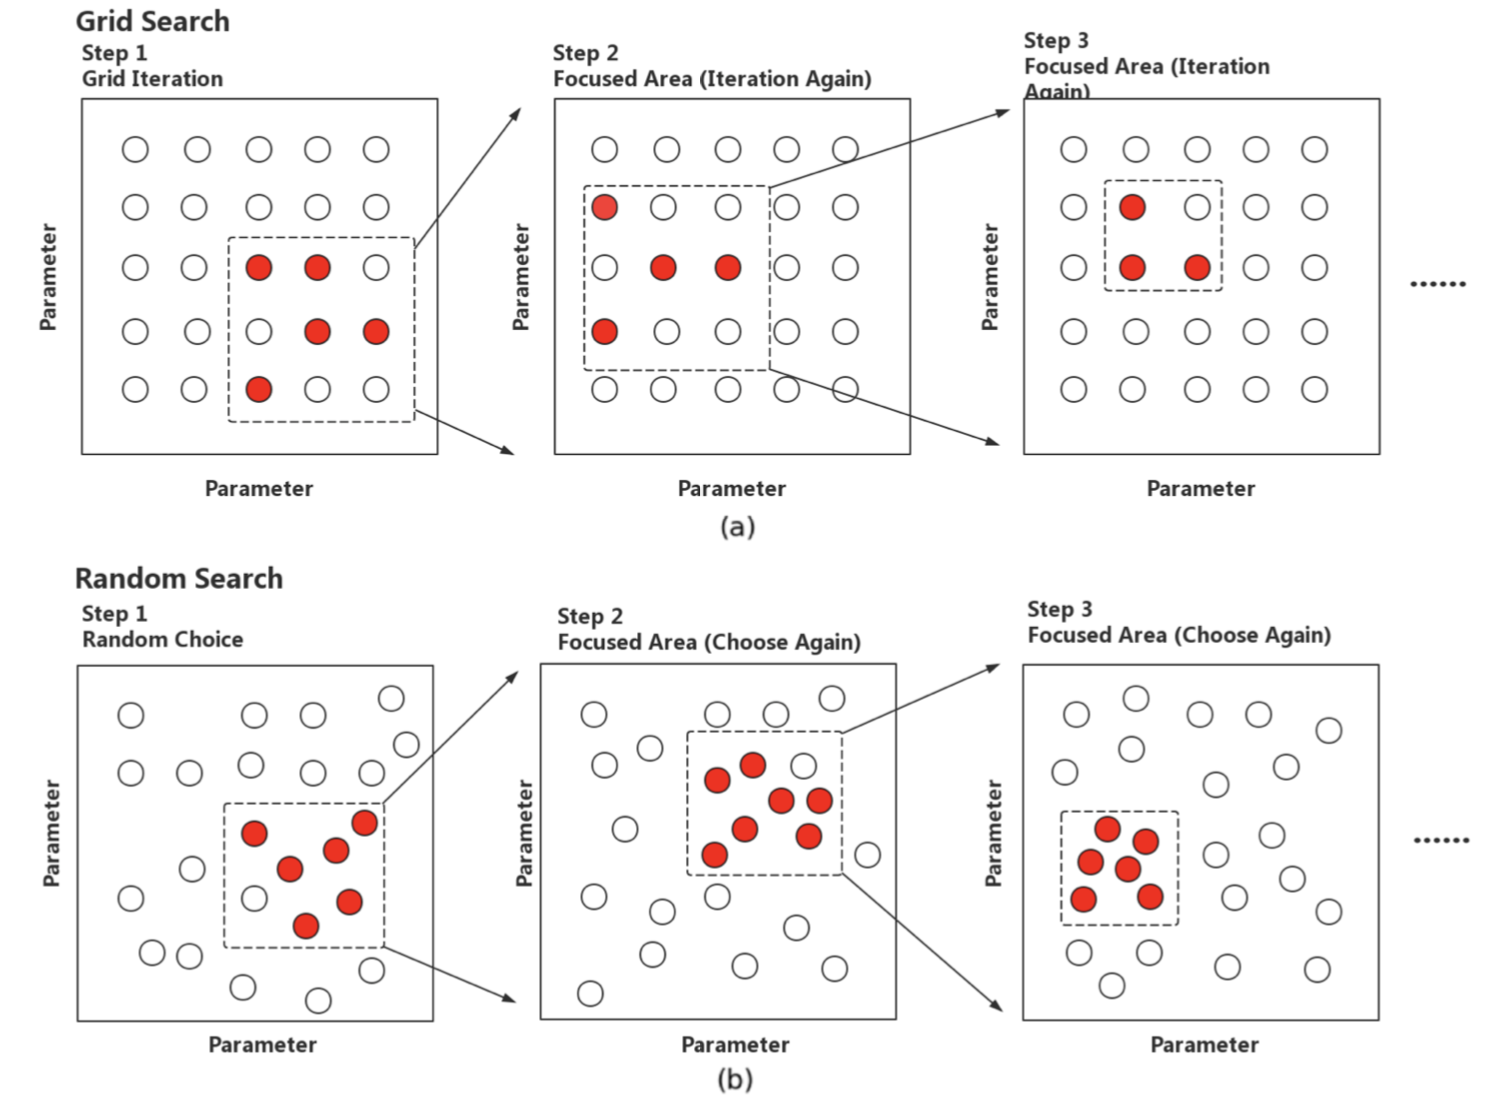
\includegraphics[scale=0.4]{example.png}
 \caption{(a) grid search and (b) random search. Red points represents the best values in each step.} 
 \label{fig:example}
\end{figure}

In most cases, since random search is more effective in practice \cite{bergstra2012random}, people use this strategy to conduct the experiment and try to find a good model. In this project, I have also chosen random search as my strategy.

\section*{Data Description}
Characterize the dataset. Describe the procedures of data preprocessing in detail. Data description can include following items:

\begin{enumerate}
    \item Number of samples and features (before and after data pre-processing).
    \item For small datasets (Up to 20 features): Compute statistics of feature values like mean, std, min, max, 25 and 95 quantiles of the dataset. 
    \item Time series plot and density plot of target.
    \item Heatmap plot to visualize the correlation among features and between features and target.
\end{enumerate}

\section*{Task I}
This part contains the results and analysis of Task I.

\subsection*{How to describe an ML-based Evaluation}

\begin{enumerate}[labelsep=0.7em, leftmargin=*]%leftmargin=0.85cm
    \item Describe precisely the data you use and the methods you employ to obtain the results. The reader should be able to reproduce the results. 
    \item Include tables and/or graphs in the description. 
    \item When you give evaluation results with numbers, 3 significant digits are generally sufficient. Providing more digits is often misleading due to uncertainties in measurements, statistics, etc. 
    \item Make the caption of a table or graph expressive, allowing the reader to grasp the main findings without reading all the surrounding text. See the caption of Figure \ref{fig:FR_NMAE_R2} as an example.
    \item  Use the same and appropriate axes scale for better comparison between plots, if possible.
    \item Use appropriate fontsize for better readability of graphs. (Example: Figure \ref{fig:FR_NMAE_R2})
    \item For a graph, address in sequence: 
        \begin{itemize}
        \item 
        Explain the axes, the points on the graph, the bars around the points, etc.
        \item 
        Describe the properties of a graph. For example, is it monotonic, does it exhibit non-continuities? etc.
        \item 
        Highlight surprising, non-intuitive behavior of the graph with respect to the evaluation.
        \item 
        Explain or suggest explanation for the observed surprising behavior.
        \end{itemize} 
\end{enumerate}
\begin{figure}[h!]
   \centering
   \subfigure[NMAE vs k for VoD service]{\label{fig:VOD_NMAE_FR}
     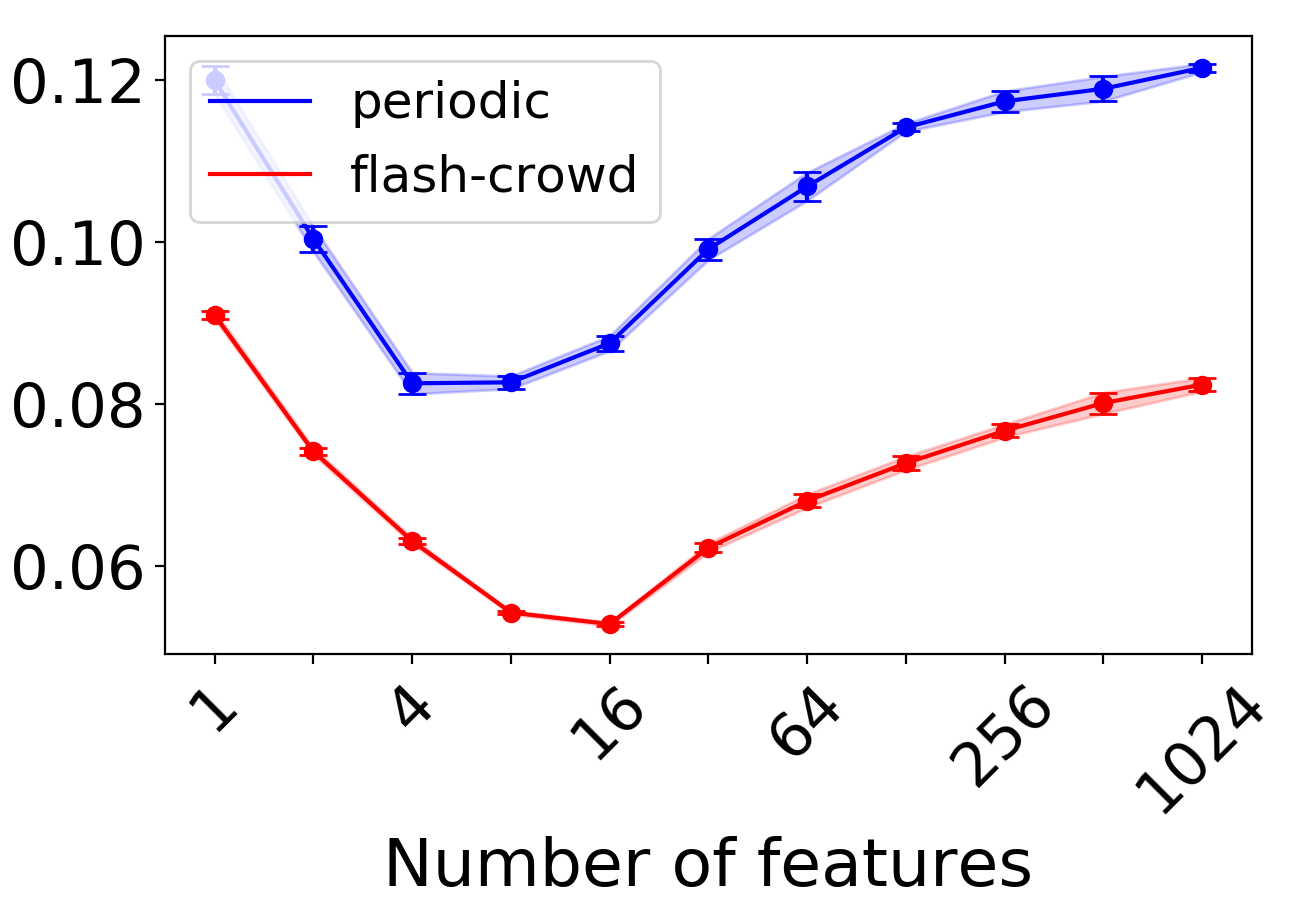
\includegraphics[width=0.32\linewidth]{FR_plots/VOD_NMAE.png}} 
   \subfigure[NMAE vs k for KV service]{\label{fig:KV_NMAE_FR}
     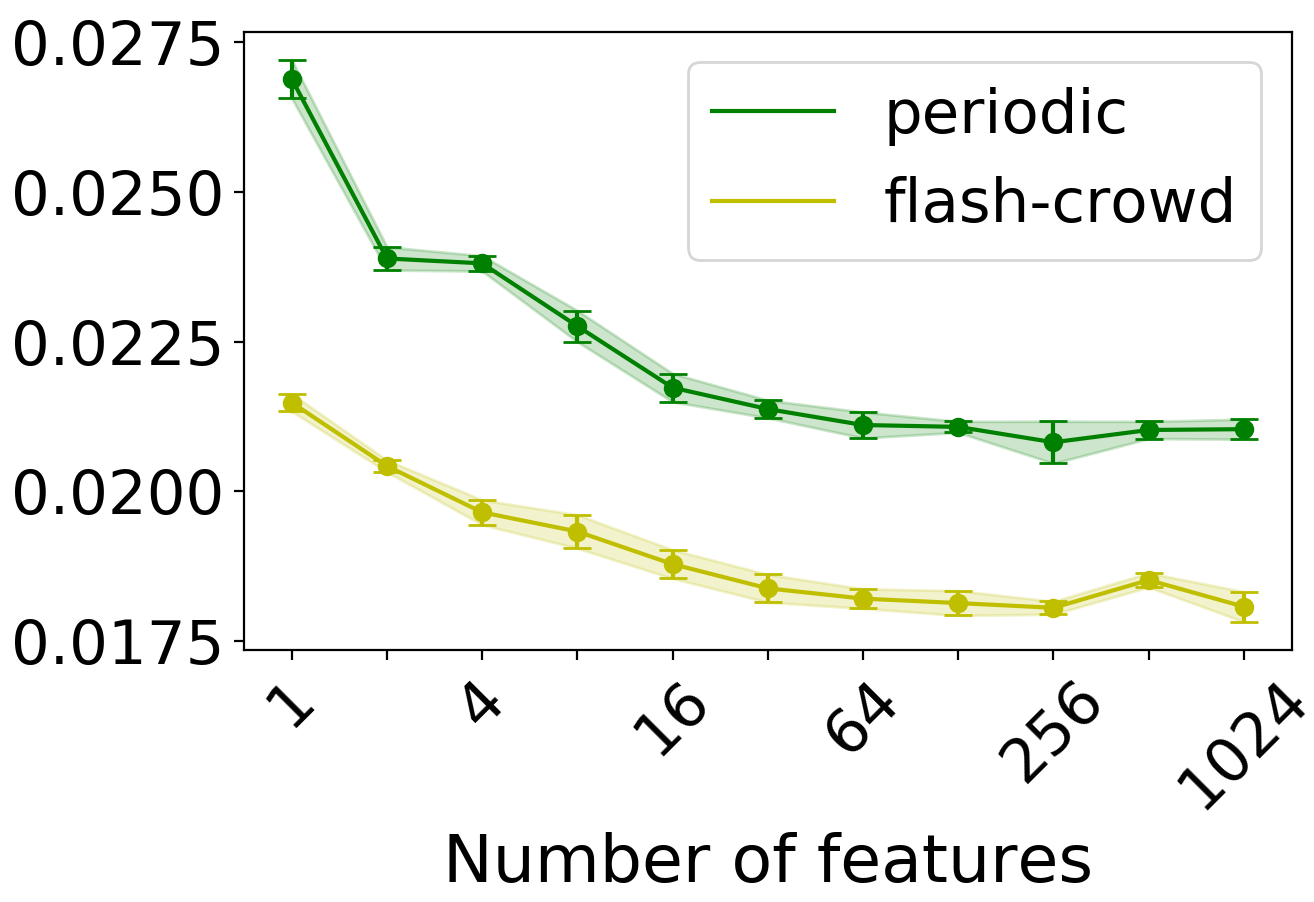
\includegraphics[width=0.32\linewidth]{FR_plots/KV_NMAE.png}}\hspace{0.15cm}
   \subfigure[$R^2$ vs k for VoD service]{\label{fig:VOD_R2_FR}
     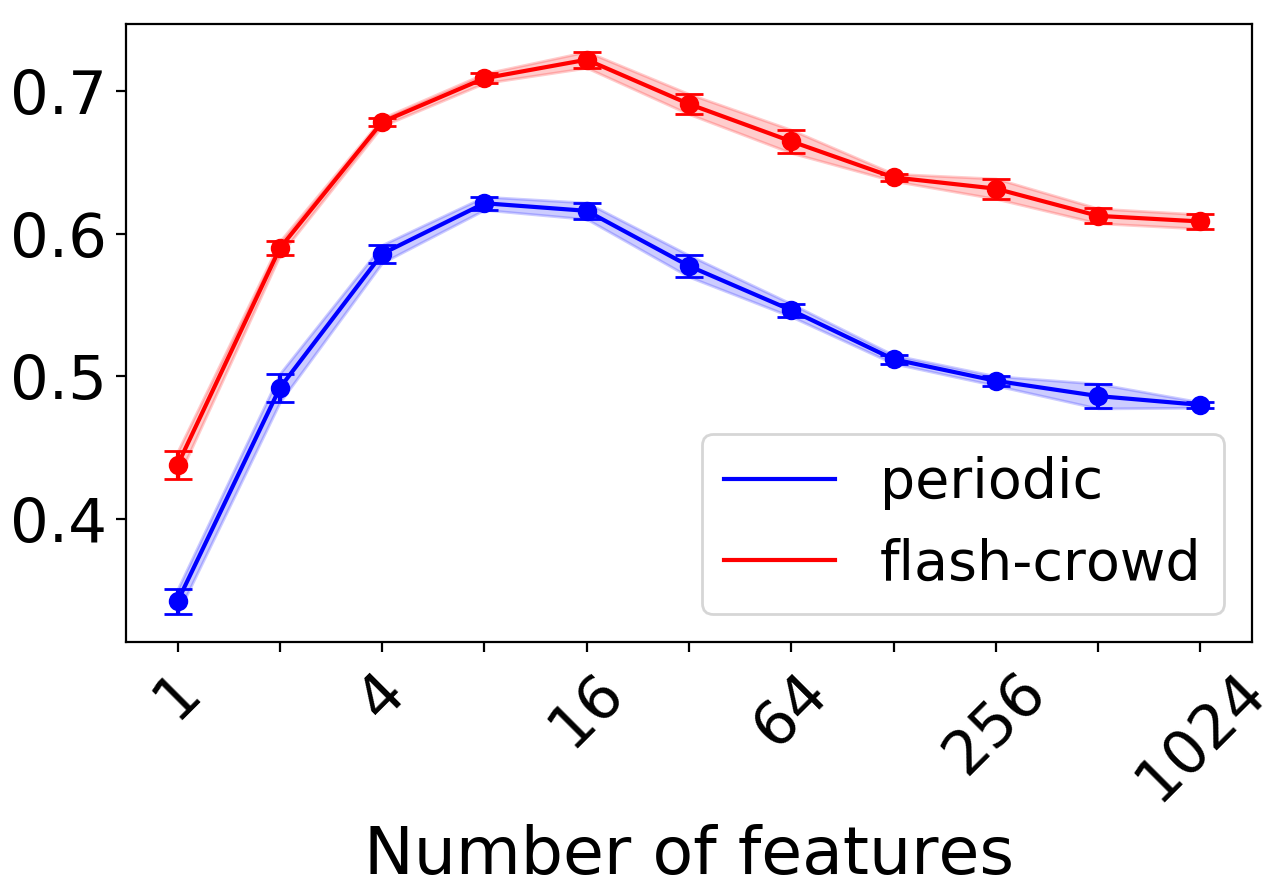
\includegraphics[width=0.32\linewidth]{FR_plots/VOD_R2.png}} 
   \subfigure[$R^2$ vs k for KV service]{\label{fig:KV_R2_FR}
     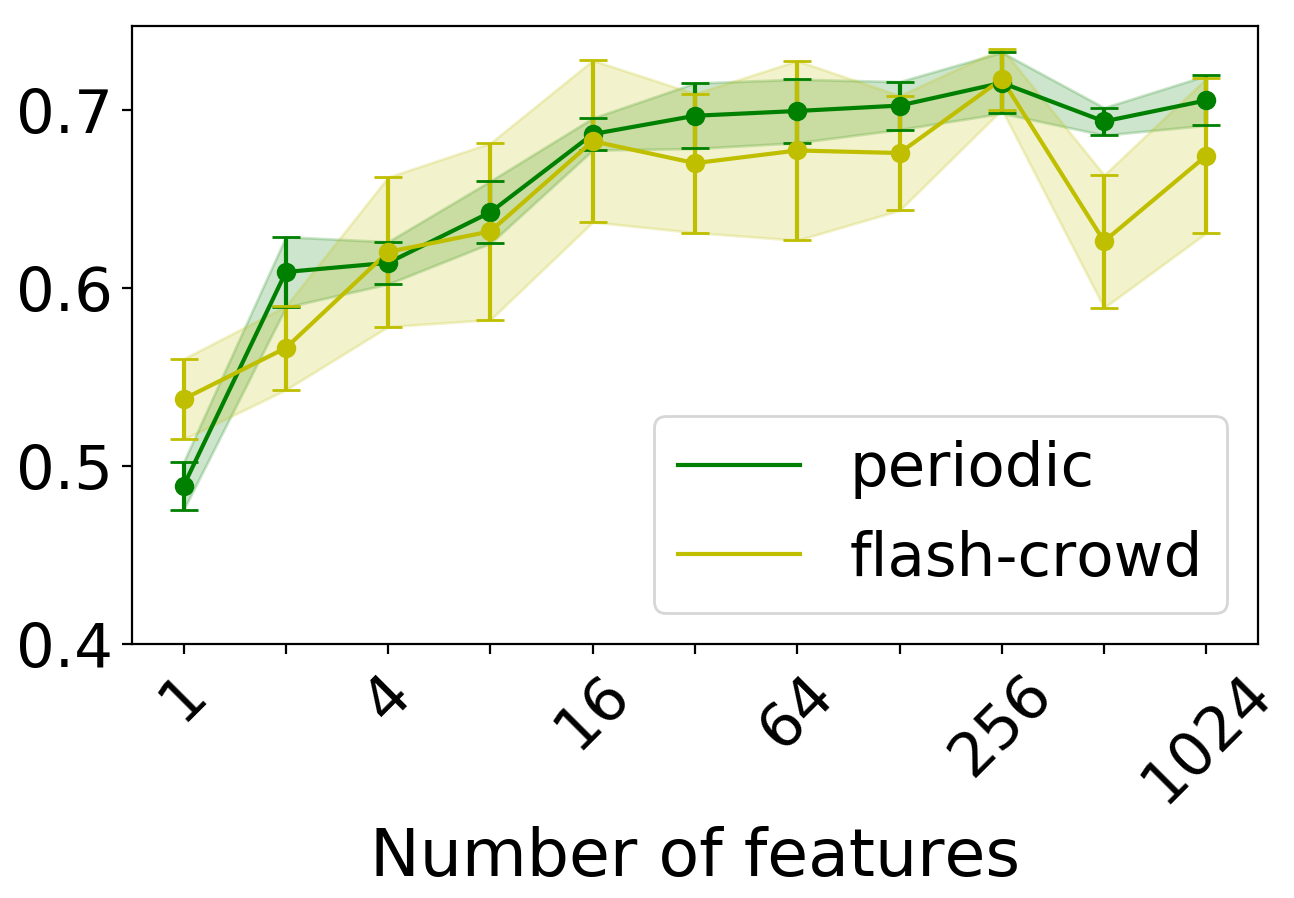
\includegraphics[width=0.32\linewidth]{FR_plots/KV_R2.png}} 
   \caption{Feature selection: Frame rate and response time prediction on the subspace spanned by the top k features. Vertical axis is prediction accuracy, horizontal axis is dimensionality of subspace.}
      \label{fig:FR_NMAE_R2}
\end{figure}


% \begin{enumerate}
% \item 
% Describe precisely the data you use and the methods you employ to obtain the results. The reader should be able to reproduce the results. 

% \item 
% Include tables and/or graphs in the description. 

% \item 
% When you give evaluation results with numbers, 3 significant digits are generally sufficient. Providing more digits is often misleading due to uncertainties in measurements, statistics, etc. 

% \item 
% Make the caption of a table or graph expressive, allowing the reader to grasp the main findings without reading all the surrounding text. See the caption of Figure \ref{fig:FR_NMAE_R2} as an example.



% \item 
% For a graph, address in sequence: 
% \begin{itemize}
% \item 
% Explain the axes, the points on the graph, the bars around the points, etc.
% \item 
% Describe the properties of a graph. For example, is it monotonic, does it exhibit non-continuities? etc.
% \item 
% Highlight surprising, non-intuitive behavior of the graph with respect to the evaluation.
% \item 
% Explain or suggest explanation for the observed surprising behavior.
% \end{itemize} 

% \end{enumerate}

\subsection*{Example:}

Figure \ref{fig:FR_NMAE_R2} shows the evaluation results for all four scenarios. We use blue curves for the scenario VoD periodic load, red for VoD flash-crowd load, green for KV periodic load, and yellow for KV flash-crowd load. Prediction accuracy is measured in $NMAE$ and $R^2$. One point on a curve represents the average value from ten-fold cross validation. The vertical bar represents the standard deviation. In most cases, the standard deviation is small and barely visible. 

The curves in Figure \ref{fig:KV_NMAE_FR} follow our expectation: when the number of dimensions increases, the prediction error falls monotonically (at least up to k=256). In contrast, Figure \ref{fig:VOD_NMAE_FR} shows that, for the VoD service, the prediction error can be significantly lower for small values of $k$ than for the full feature space $X$ where $k=1409$. This is surprising and suggests that many features do not contribute to an accurate prediction of the frame rate and actually reduce accuracy. For VoD, the optimal value of $k$ with the smallest prediction error is between 8 and 16, while for KV the optimal $k$ is around 256. 

 

\section*{Task II}
This part contains the results and analysis of Task II.

...

\section*{Discussion}
For each of the above sections, list and discuss the key points. Optionally, suggest further investigations one can conduct to achieve the project objectives.


\bibliographystyle{ieeetr}

\bibliography{references}

\end{document}

